\imagefigure{
    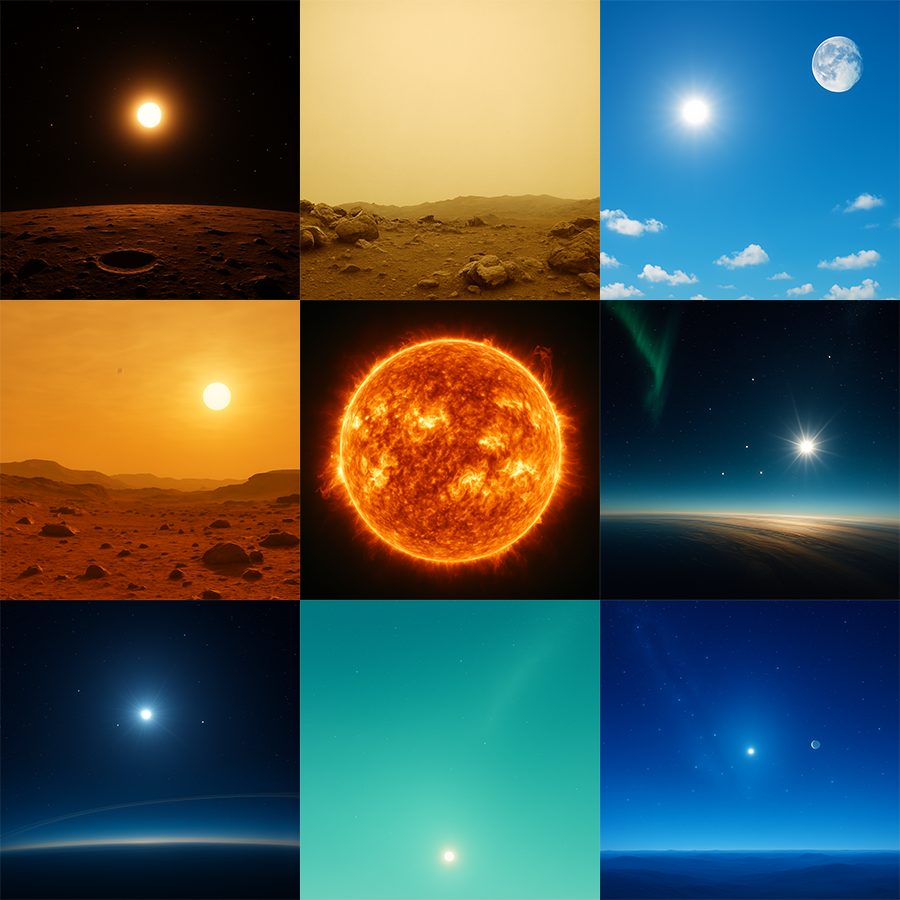
\includegraphics[width=0.8\textwidth]{27_PlanetarySkyColors/SKIES.png} 
}{
Nine simulated daytime skies from each planet in the Solar System, arranged heliocentrically around the Sun in a 3$\times$3 grid. The rows (left to right, top to bottom) correspond to: Mercury, Venus, Earth; Mars, Sun, Jupiter; Saturn, Uranus, Neptune. Each panel reflects sky color, atmospheric scattering, and visible celestial features such as moons, rings, and the Sun's apparent size, as modeled for surface or high-atmosphere observation.
}
